\section{SELECCIÓN DE LA ARQUITECTURA TECNOLÓGICA} \label{sec:4_seleccion_arquitectura_tecnologica}
\hypertarget{sec:4_seleccion_arquitectura_tecnologica}{}

En esta sección se presentan las decisiones tomadas en cuanto a la arquitectura tecnológica del proyecto, el análisis de las alternativas distintas alternativas se 
puede consultar en la sección \coloredUnderline{\hyperlink{sec:3_2-Alternativas-solucion}{\ref*{sec:3_2-Alternativas-solucion}: \nameref*{sec:3_2-Alternativas-solucion}}}.


El proyecto está diseñado para tener una clara distinción entre el \textit{frontend} y el \textit{backend}, lo cual facilita la escalabilidad y el mantenimiento del sistema. 
Se ha optado por implementar la arquitectura de tipo REST API y Web App. El módulo REST API, es decir, el \textit{backend} será responsable de la lógica de negocio, 
mientras que el módulo Web App, \textit{frontend}, gestionará la presentación de la información. 

Esta estructura permite que el desarrollo del \textit{frontend} se realice de manera independiente al \textit{backend}, permitiendo modificaciones en uno sin afectar al otro. 
La comunicación entre el \textit{frontend} y el \textit{backend} se llevará a cabo mediante peticiones HTTP, como se ilustra en la \coloredUnderline{\hyperlink{fig:arquitectura_rest}{Figura \ref*{fig:arquitectura_rest}: \nameref*{fig:arquitectura_rest}}}.


\begin{figure}[H]
    \centering
    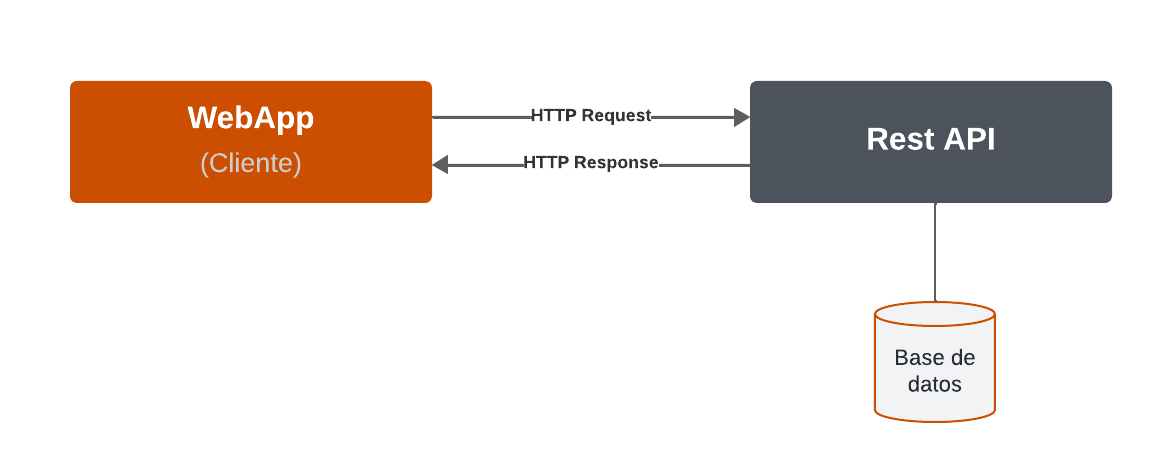
\includegraphics[width=0.7\textwidth]{figures/4-Arquitectura-tecnologica/4_REST.png}
    \caption{Arquitectura REST API y Web App}
    \label{fig:arquitectura_rest}
    \hypertarget{fig:arquitectura_rest}{}
\end{figure}


Se han seleccionado las siguientes tecnologías como alternativas de solución: Node.js con Express para el backend, React.js para el frontend, y MongoDB Atlas como base 
de datos.

Estas decisiones conforman una arquitectura \coloredUnderline{\href{https://www.mongodb.com/resources/languages/mern-stack}{\textbf{MERN}}} (MongoDB, Express, React, Node.js), ejemplificada en la \coloredUnderline{\hyperlink{fig:arquitectura_mern}{Figura \ref*{fig:arquitectura_mern}: \nameref*{fig:arquitectura_mern}}}. 

Esta arquitectura presenta diversas ventajas, tales como la familiaridad de los desarrolladores con las tecnologías involucradas, el amplio soporte y documentación disponibles debido a su uso común en el desarrollo de aplicaciones web actuales,
y la facilidad de integración entre las tecnologías.

Si bien esta arquitectura se fundamenta en el lenguaje de programación JavaScript, se ha decidido adoptar TypeScript. Este lenguaje es una extensión de JavaScript que introduce tipado estático al lenguaje, 
lo que no solo facilita la detección de errores durante la compilación, sino que también contribuye significativamente a la mejora de la calidad del código y a la comprensión de este.


\begin{figure}[H]
    \centering
    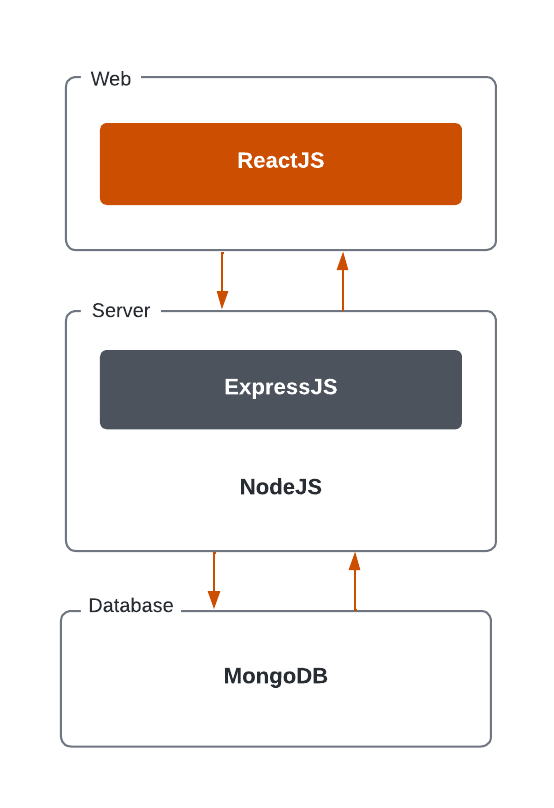
\includegraphics[width=0.4\textwidth]{figures/4-Arquitectura-tecnologica/4_MERN2.png}
    \caption{MERN Stack: MongoDB, Express, React, Node.js}
    \label{fig:arquitectura_mern}
    \hypertarget{fig:arquitectura_mern}{}
\end{figure}

Para el despliegue de la aplicación se ha optado por utilizar la plataforma de servicios en la nube de Microsoft, Azure.
Esta elección se complementa con el uso de \coloredUnderline{\href{https://github.com/features/actions}{GitHub Actions}}
para la implementación de procesos de integración continua, 
permitiendo así un desarrollo ágil y sistemático. Como se ha comentado anteriormente, se incorporará MongoDB Atlas para gestionar la base de datos en la nube, aprovechando su capacidad de escalabilidad 
y flexibilidad. Por último, se utilizará \coloredUnderline{\href{https://www.docker.com/}{Docker}} 
para la contenerización de la aplicación, facilitando la portabilidad y la consistencia del entorno de ejecución a través de diferentes infraestructuras de despliegue. 
Este enfoque integrado asegura una arquitectura robusta y eficiente para el despliegue de la aplicación en un entorno de nube.